\begin{tikzpicture}
	\pgfplotsset{/tikz/font={\small}}
	\begin{axis}[
		grid=both,
		width=1.0\textwidth,
		height=0.3\textheight,
		ytick={0,200,...,1400},
		y tick label style={
		/pgf/number format/.cd,
		fixed,
		fixed zerofill,
		precision=0,
		set thousands separator={\thinspace}},
		% y dir=reverse,
		ymax=1400, ymin=0,
		ylabel={Number of blocks ($\times1000$)},
		xlabel={\acfp{IPM}},
		% enlargelimits=0.15,
		enlarge y limits=false,
		enlarge x limits=0.04,
		legend style={at={(0.5,-0.20)},
		anchor=north,legend columns=-1},
		ybar interval,
		% bar width=2pt,
		% bar shift=10pt
		xtick=data,
		xtick align=inside,
		% nodes near coords,
		% xlabel={Sequences},
		% xlabel near ticks,
		% x tick label style={rotate=-60,anchor=west},
		]
		\addlegendentry{$4\times4$}
		\addplot coordinates { % values have beed divided by 1000
		(0, 1364.213)
		(1,  724.842)
		(2,   56.522)
		(3,   61.151)
		(4,   55.249)
		(5,   64.906)
		(6,   98.925)
		(7,  122.995)
		(8,  273.925)
		(9,  416.868)
		(10, 726.798)
		(11, 731.229)
		(12, 286.635)
		(13, 248.812)
		(14, 307.531)
		(15, 214.435)
		(16, 152.227)
		(17, 162.321)
		(18,  71.355)
		(19, 107.414)
		(20,  91.012)
		(21,  98.337)
		(22, 126.187)
		(23, 128.947)
		(24, 149.842)
		(25, 307.650)
		(26, 738.189)
		(27, 276.359)
		(28, 150.686)
		(29, 116.680)
		(30, 105.906)
		(31,  75.812)
		(32,  72.256)
		(33,  75.184)
		(34,  53.216)
		(35, 0)
		};

		\addlegendentry{$8\times8$}
		\addplot coordinates { % values have beed divided by 1000
		(0, 1215.199)
		(1,  689.480)
		(2,   81.395)
		(3,   29.846)
		(4,   33.355)
		(5,   42.454)
		(6,   57.356)
		(7,   75.645)
		(8,  151.422)
		(9,  331.490)
		(10, 426.614)
		(11, 428.937)
		(12, 159.159)
		(13, 149.122)
		(14, 128.801)
		(15,  90.122)
		(16,  58.692)
		(17,  40.322)
		(18, 109.448)
		(19,  27.579)
		(20,  33.682)
		(21,  44.409)
		(22,  49.680)
		(23,  63.084)
		(24,  86.251)
		(25, 239.589)
		(26, 540.578)
		(27, 217.064)
		(28,  89.107)
		(29,  66.923)
		(30,  50.982)
		(31,  43.990)
		(32,  37.089)
		(33,  32.193)
		(34,  72.435)
		(35,0)
		};
	\end{axis}
\end{tikzpicture}
